% This template is borrowed from the Reed College LaTeX thesis template. Most of the work
% for the document class was done by Sam Noble (SN), as well as this
% template. Later comments etc. by Ben Salzberg (BTS). Additional
% restructuring and APA support by Jess Youngberg (JY).
% Your comments and suggestions are more than welcome; please email
% them to cus@reed.edu
%
% See http://web.reed.edu/cis/help/latex.html for help. There are a
% great bunch of help pages there, with notes on
% getting started, bibtex, etc. Go there and read it if you're not
% already familiar with LaTeX.
%
% Any line that starts with a percent symbol is a comment.
% They won't show up in the document, and are useful for notes
% to yourself and explaining commands.
% Commenting also removes a line from the document;
% very handy for troubleshooting problems. -BTS

% As far as I know, this follows the requirements laid out in
% the 2002-2003 Senior Handbook. Ask a librarian to check the
% document before binding. -SN

%%
%% Preamble
%%
% \documentclass{<something>} must begin each LaTeX document
\documentclass[12pt,twoside]{deuthesis}
% Packages are extensions to the basic LaTeX functions. Whatever you
% want to typeset, there is probably a package out there for it.
% Chemistry (chemtex), screenplays, you name it.
% Check out CTAN to see: http://www.ctan.org/
%%
\usepackage{graphicx,latexsym}
\usepackage{amsmath}
\usepackage{amssymb,amsthm}
\usepackage{longtable,booktabs,setspace}
\usepackage{chemarr} %% Useful for one reaction arrow, useless if you're not a chem major
\usepackage[hyphens]{url}
% Added by CII
\usepackage{hyperref}
\usepackage{lmodern}
\usepackage{float}
\floatplacement{figure}{H}
% End of CII addition
\usepackage{rotating}

% Next line commented out by CII
%%% \usepackage{natbib}
% Comment out the natbib line above and uncomment the following two lines to use the new
% biblatex-chicago style, for Chicago A. Also make some changes at the end where the
% bibliography is included.
%\usepackage{biblatex-chicago}
%\bibliography{thesis}


% Added by CII (Thanks, Hadley!)
% Use ref for internal links
\renewcommand{\hyperref}[2][???]{\autoref{#1}}
\def\chapterautorefname{Chapter}
\def\sectionautorefname{Section}
\def\subsectionautorefname{Subsection}
% End of CII addition

% Added by CII
\usepackage{caption}
\captionsetup{width=5in}
% End of CII addition

% \usepackage{times} % other fonts are available like times, bookman, charter, palatino

% Syntax highlighting #22
  \usepackage{color}
  \usepackage{fancyvrb}
  \newcommand{\VerbBar}{|}
  \newcommand{\VERB}{\Verb[commandchars=\\\{\}]}
  \DefineVerbatimEnvironment{Highlighting}{Verbatim}{commandchars=\\\{\}}
  % Add ',fontsize=\small' for more characters per line
  \usepackage{framed}
  \definecolor{shadecolor}{RGB}{248,248,248}
  \newenvironment{Shaded}{\begin{snugshade}}{\end{snugshade}}
  \newcommand{\AlertTok}[1]{\textcolor[rgb]{0.94,0.16,0.16}{#1}}
  \newcommand{\AnnotationTok}[1]{\textcolor[rgb]{0.56,0.35,0.01}{\textbf{\textit{#1}}}}
  \newcommand{\AttributeTok}[1]{\textcolor[rgb]{0.13,0.29,0.53}{#1}}
  \newcommand{\BaseNTok}[1]{\textcolor[rgb]{0.00,0.00,0.81}{#1}}
  \newcommand{\BuiltInTok}[1]{#1}
  \newcommand{\CharTok}[1]{\textcolor[rgb]{0.31,0.60,0.02}{#1}}
  \newcommand{\CommentTok}[1]{\textcolor[rgb]{0.56,0.35,0.01}{\textit{#1}}}
  \newcommand{\CommentVarTok}[1]{\textcolor[rgb]{0.56,0.35,0.01}{\textbf{\textit{#1}}}}
  \newcommand{\ConstantTok}[1]{\textcolor[rgb]{0.56,0.35,0.01}{#1}}
  \newcommand{\ControlFlowTok}[1]{\textcolor[rgb]{0.13,0.29,0.53}{\textbf{#1}}}
  \newcommand{\DataTypeTok}[1]{\textcolor[rgb]{0.13,0.29,0.53}{#1}}
  \newcommand{\DecValTok}[1]{\textcolor[rgb]{0.00,0.00,0.81}{#1}}
  \newcommand{\DocumentationTok}[1]{\textcolor[rgb]{0.56,0.35,0.01}{\textbf{\textit{#1}}}}
  \newcommand{\ErrorTok}[1]{\textcolor[rgb]{0.64,0.00,0.00}{\textbf{#1}}}
  \newcommand{\ExtensionTok}[1]{#1}
  \newcommand{\FloatTok}[1]{\textcolor[rgb]{0.00,0.00,0.81}{#1}}
  \newcommand{\FunctionTok}[1]{\textcolor[rgb]{0.13,0.29,0.53}{\textbf{#1}}}
  \newcommand{\ImportTok}[1]{#1}
  \newcommand{\InformationTok}[1]{\textcolor[rgb]{0.56,0.35,0.01}{\textbf{\textit{#1}}}}
  \newcommand{\KeywordTok}[1]{\textcolor[rgb]{0.13,0.29,0.53}{\textbf{#1}}}
  \newcommand{\NormalTok}[1]{#1}
  \newcommand{\OperatorTok}[1]{\textcolor[rgb]{0.81,0.36,0.00}{\textbf{#1}}}
  \newcommand{\OtherTok}[1]{\textcolor[rgb]{0.56,0.35,0.01}{#1}}
  \newcommand{\PreprocessorTok}[1]{\textcolor[rgb]{0.56,0.35,0.01}{\textit{#1}}}
  \newcommand{\RegionMarkerTok}[1]{#1}
  \newcommand{\SpecialCharTok}[1]{\textcolor[rgb]{0.81,0.36,0.00}{\textbf{#1}}}
  \newcommand{\SpecialStringTok}[1]{\textcolor[rgb]{0.31,0.60,0.02}{#1}}
  \newcommand{\StringTok}[1]{\textcolor[rgb]{0.31,0.60,0.02}{#1}}
  \newcommand{\VariableTok}[1]{\textcolor[rgb]{0.00,0.00,0.00}{#1}}
  \newcommand{\VerbatimStringTok}[1]{\textcolor[rgb]{0.31,0.60,0.02}{#1}}
  \newcommand{\WarningTok}[1]{\textcolor[rgb]{0.56,0.35,0.01}{\textbf{\textit{#1}}}}

% To pass between YAML and LaTeX the dollar signs are added by CII
\title{PROJE BAŞLIĞI}
%\author{Pelin PEKERMerve AKEdanur Binnaz DURSUNAhmet ÇALI} %Tek yazar için
\author{Pelin PEKER \\ Merve AK \\ Edanur Binnaz DURSUN \\ Ahmet ÇALI} %Çok yazar için
% The month and year that you submit your FINAL draft TO THE LIBRARY (May or December)
\date{Nisan 2024}
\division{İSTATİSTİK BÖLÜMÜ}
\advisor{Dr.~Engin YILDIZTEPE}
\institution{FEN FAKÜLTESİ}
\degree{Bitirme Projesi Raporu}
%If you have two advisors for some reason, you can use the following
% Uncommented out by CII
% End of CII addition

%%% Remember to use the correct department!
\department{İstatistik Bölümü}
% if you're writing a thesis in an interdisciplinary major,
% uncomment the line below and change the text as appropriate.
% check the Senior Handbook if unsure.
%\thedivisionof{The Established Interdisciplinary Committee for}
% if you want the approval page to say "Approved for the Committee",
% uncomment the next line
%\approvedforthe{Committee}

% Added by CII
%%% Copied from knitr
%% maxwidth is the original width if it's less than linewidth
%% otherwise use linewidth (to make sure the graphics do not exceed the margin)
\makeatletter
\def\maxwidth{ %
  \ifdim\Gin@nat@width>\linewidth
    \linewidth
  \else
    \Gin@nat@width
  \fi
}
\makeatother

\renewcommand{\contentsname}{Table of Contents}
% End of CII addition

\setlength{\parskip}{0pt}

% Added by CII

\providecommand{\tightlist}{%
  \setlength{\itemsep}{0pt}\setlength{\parskip}{0pt}}

\Acknowledgements{
Tüm çalışma süresince yönlendiriciliği, katkıları ve yardımları ile yanımızda olan danışmanımız Dr.~Engin YILDIZTEPE 'ye ve böyle bir çalışmayı yapmamız için bize fırsat tanıyan Dokuz Eylül Üniversitesi Fen Fakültesi İstatistik Bölümüne teşekkür ederiz.\\
\strut \\
\strut \\
Pelin PEKER\\
Merve AK\\
Edanur Binnaz DURSUN\\
Ahmet ÇALI\\
}

\Dedication{

}

\Preface{
``PROJE BAŞLIĞI'' başlıklı bitirme projesi raporu tarafıgitmdan okunmuş, kapsamı ve niteliği açısından bir Bitirme Projesi raporu olarak kabul edilmiştir.\\
\strut \\
\strut \\
Dr.~Engin YILDIZTEPE
}

\AbstractTR{
Özet, çalışmanın önemini ve faydasını anlatan bir bölüm degildir. Çalısmayı ana
hatlarıyla anlatacak ve 300 kelimeyi aşmayacak şekilde hazırlanmalıdır. En az üç en
çok beş anahtar kelime ilgili yere yazılmalıdır.

\par

ikinci paragraf buradan başlar\\
\strut \\
\textbf{Anahtar Kelimeler:} anahtar kelime 1, anahtar kelime 2, anahtar kelime 3
}

\Abstract{
The preface pretty much says it all.

\par

Second paragraph of abstract starts here.\\
\strut \\
\textbf{Keywords:} keyword1, keyword2, keyword3
}


% End of CII addition
%%
%% End Preamble
%%
%

\begin{document}

% Everything below added by CII
  \maketitle

\frontmatter % this stuff will be roman-numbered
\pagestyle{empty} % this removes page numbers from the frontmatter

\begin{preface}
	``PROJE BAŞLIĞI'' başlıklı bitirme projesi raporu tarafıgitmdan okunmuş, kapsamı ve niteliği açısından bir Bitirme Projesi raporu olarak kabul edilmiştir.\\
\strut \\
\strut \\
Dr.~Engin YILDIZTEPE
\end{preface}

  \begin{acknowledgements}
    Tüm çalışma süresince yönlendiriciliği, katkıları ve yardımları ile yanımızda olan danışmanımız Dr.~Engin YILDIZTEPE 'ye ve böyle bir çalışmayı yapmamız için bize fırsat tanıyan Dokuz Eylül Üniversitesi Fen Fakültesi İstatistik Bölümüne teşekkür ederiz.\\
    \strut \\
    \strut \\
    Pelin PEKER\\
    Merve AK\\
    Edanur Binnaz DURSUN\\
    Ahmet ÇALI\\
  \end{acknowledgements}

\begin{abstractTR}
	Özet, çalışmanın önemini ve faydasını anlatan bir bölüm degildir. Çalısmayı ana
hatlarıyla anlatacak ve 300 kelimeyi aşmayacak şekilde hazırlanmalıdır. En az üç en
çok beş anahtar kelime ilgili yere yazılmalıdır.

\par

ikinci paragraf buradan başlar\\
\strut \\
\textbf{Anahtar Kelimeler:} anahtar kelime 1, anahtar kelime 2, anahtar kelime 3
\end{abstractTR}

\begin{abstract}
	The preface pretty much says it all.

\par

Second paragraph of abstract starts here.\\
\strut \\
\textbf{Keywords:} keyword1, keyword2, keyword3
\end{abstract}


  \hypersetup{linkcolor=black}
  \setcounter{tocdepth}{2}
  \tableofcontents

  \listoftables

  \listoffigures


% This was added by EY
\newlength{\cslhangindent}
\setlength{\cslhangindent}{1.5em}
\newenvironment{CSLReferences}%
  {}%
  {\par}
\newenvironment{cslreferences}%
  {}%
  {\par}

\mainmatter % here the regular arabic numbering starts
\pagestyle{fancyplain} % turns page numbering back on

\hypertarget{giriux15f}{%
\chapter*{GİRİŞ}\label{giriux15f}}
\addcontentsline{toc}{chapter}{GİRİŞ}

Değişim noktası, veri setinde ani ve beklenmedik bir değişikliği ifade eden bir konum olarak tanımlanır. Bu noktalar genellikle bir desenin, trendin, varyansın veya diğer istatistiksel özelliklerin birdenbire ve belirgin bir şekilde değiştiği yerlerdir. Değişim noktası kestirimi; haberleşme, biyomedikal alanlar, konuşma sinyalleri işleme, sismik veri analizi, istatistiksel süreç kontrolü, finansal veri analizi gibi çeşitli alanlarda yaygın olarak kullanılan bir yöntemdir. Bu kestirim probleminin çözümü için çeşitli istatistiksel sinyal işleme teknikleri geliştirilmiştir. Veri dağılımının bilindiği ve bilinmediği durumlarda kullanılan yöntemler, parametrik ve parametrik olmayan olarak sınıflandırılır. Ölçümlere ait dağılım fonksiyonunun bilinmesi, genellikle parametrik değişim noktası kestirim yöntemleriyle zor problemlerde bile başarılı sonuçlar elde edilmesini sağlar. Ancak bu bilgi her zaman mevcut olmayabilir ve bu durumda parametrik olmayan yöntemlere başvurulur.

Örneğin, bir perakende satış veri setinde, bir ürünün satışlarının aniden artması veya azalması bir değişim noktasını temsil edebilir. Endüstriyel süreçlerde, üretim hattındaki bir arıza nedeniyle üretimde ani bir düşüş de bir değişim noktası olabilir. Finansal piyasalarda, bir hisse senedinin değerinde ani bir değişiklik veya trendin tersine dönmesi de bir değişim noktasını işaret edebilir. Değişim noktalarını tespit etmek için istatistiksel analiz, zaman serisi analizi, makine öğrenimi gibi teknikler kullanılır. Bayes faktörü, kümülatif toplam, anomalilerin tespiti gibi istatistiksel kriterler, değişim noktalarını belirlemede kullanılan araçlardan bazılarıdır. Bu teknikler, veriyi segmentlere ayırır ve her bir segmentin içindeki istatistiksel özellikleri değerlendirerek değişim noktalarını tanımlar.

Bu analizler, veri setindeki önemli değişiklikleri objektif bir şekilde belirleyerek, kullanıcılara olayları anlama ve gelecekteki eğilimleri tahmin etme konusunda yardımcı olabilir. Bu sayede, değişim noktalarının belirlenmesi, karar verme süreçlerini destekleyerek daha bilinçli ve stratejik adımlar atılmasına imkan tanır.

\hypertarget{Bolum2}{%
\chapter{DEĞİŞİM NOKTASI}\label{Bolum2}}

\hypertarget{tek-deux11fiux15fim-noktasi-tespiti}{%
\section{TEK DEĞİŞİM NOKTASI TESPİTİ}\label{tek-deux11fiux15fim-noktasi-tespiti}}

Tek değişim noktası tespiti, bir veri setinde yalnızca bir değişim noktasının varlığını tespit etmeye odaklanan istatistiksel bir analiz yöntemidir. Bu tür analizler genellikle zaman serileri, süreç kontrolü, finansal veriler gibi çeşitli alanlarda kullanılır. Temel hedef, veri setindeki bu değişim noktasını tanımlamak ve bu noktada meydana gelen ani değişikliği belirlemektir.

Tek değişim noktası tespiti, bir zaman serisinde veya veri setinde belirli bir anın, örneğin bir trendin başlangıcı veya bir olayın etkisi gibi bir değişiklik noktasını belirlemek için kullanılır. Bu analiz genellikle istatistiksel yöntemler, matematiksel modeller veya makine öğrenimi algoritmaları kullanılarak gerçekleştirilir. Bu yöntemler, veri setindeki değişim noktasının istatistiksel olarak anlamlı olup olmadığını değerlendirir ve belirli bir ölçüye dayanarak değişim noktasını tanımlar.
Bu tür analizler, anormal durumları tespit etmek, süreçlerdeki değişiklikleri anlamak veya zaman içindeki önemli olayları belirlemek gibi bir dizi uygulama alanında kullanılır. Örneğin, endüstriyel süreçlerde bir makinenin arızasının başlangıcını belirlemek veya finansal piyasalardaki bir trend değişikliğini saptamak gibi durumlar, tek değişim noktası tespiti analizine örnek olabilir. Bu yöntemler, veri analizi ve karar verme süreçlerinde bilinçli ve stratejik adımlar atılmasına yardımcı olabilir, çünkü belirli bir değişim noktasının tanımlanması, olayların anlaşılmasını ve gelecekteki trendlerin tahmin edilmesini destekleyebilir.

Tek bir değişim noktasının tespiti için hipotez testi bir olasılık oranı tabanlı yaklaşımla formüle edilebilir. Burada, H0 null hipotezi, değişim noktasının olmadığına (m = 0) karşılık gelirken, alternatif hipotez H1 tek bir değişim noktasına (m = 1) karşılık gelir.

Bu hipotezi test etmek için olasılık oranı test istatistiği, genel bir hipotez tabanlı yaklaşımı kullanır. İlk olarak, Hinkley (1970) tarafından önerilen bu yöntem, asimptotik dağılımı türetilen bir olasılık tabanlı yaklaşımı benimser. Bu yaklaşım, normal olarak dağılmış gözlemler içindeki ortalama değişikliği için olasılık oranı test istatistiğini hesaplar.

Jen ve Gupta (1987) tarafından yapılan genişletme ile bu olasılık tabanlı yaklaşım, normal olarak dağılmış gözlemler içindeki varyans değişiklikleri için de geçerli bir test istatistiği sağlar.

Bu yöntemler, belirli bir değişim noktasının varlığını istatistiksel olarak değerlendirmek ve bu değişim noktasının ne zaman gerçekleştiğini belirlemek için kullanılır. Bu analizler, veri setindeki belirli bir noktadaki değişikliklerin anlamlılığını değerlendirerek, değişim noktasının varlığını istatistiksel olarak doğrulamaya yöneliktir.

Null hipotezi için maksimum log-olabilirlik, \(\log p(y_{1:n}|\hat{\theta})\) şeklinde ifade edilir, burada \(p(\cdot)\) verilerin dağılımıyla ilişkilendirilen olasılık yoğunluk fonksiyonudur ve \(\hat{\theta}\) parametrelerin maksimum olabilirlik tahminidir.

Alternatif hipotez altında, \(\tau_1\) ile bir değişim noktası içeren bir modeli ele alalım, burada \(\tau_1 \in {1, 2, \dots, n - 1}\). Bu durumda, belirli bir \(\tau_1\) için maksimum log-olabilirlik şu şekildedir: \(ML(\tau_1) = \log p(y_{1:\tau_1}|\hat{\theta}_1) + \log p(y_{(\tau_1+1):n}|\hat{\theta}_2)\). Değişim noktasının doğası göz önüne alındığında, alternatif hipotez altındaki maksimum log-olabilirlik değeri basitçe \(\max{\tau_1} ML(\tau_1)\) olarak ifade edilir, burada maksimum tüm olası değişim noktası konumları için alınır. Test istatistiği şu şekildedir: \(\lambda = 2\tau_1 ML(\tau_1) - \log p(y_{1:n}|\hat{\theta})_{\max}\).

Bu test, \(\lambda > c\) ise null hipotezi reddedilir şeklinde bir eşik değeri \(c\) seçerek yapılır. Eğer null hipotezi reddedilirse, yani bir değişim noktası algılanırsa, onun pozisyonunu \(\hat{\tau}_1\) olarak tahmin ederiz, bu değer \(ML(\tau_1)\)'i maksimize eden \(\tau_1\) değeridir. Bu parametre için uygun değer \(c\) henüz açık bir araştırma sorusudur ve farklı değişim tipleri altında \(p\) değerleri ve diğer bilgi kriterleri oluşturan birkaç yazar bulunmaktadır (Birgé ve Massart, 2007; Chen, Gupta ve Gupta, 2000; Guyon ve Yao, 1999; Lavielle, 2005).

Açıkça görülmektedir ki, olabilirlik test istatistiği basitçe \(m\) segmentlerinin her biri için olasılığı toplamak suretiyle birden fazla değişime genişletilebilir. Sorun, tüm olası \(\tau_{1:m}\) kombinasyonları üzerinde \(ML(\tau_{1:m})\)'in maksimumunu belirlemeye dönüşür.

\hypertarget{line-breaks}{%
\section{Line breaks}\label{line-breaks}}

Make sure to add white space between lines if you'd like to start a new paragraph. Look at what happens below in the outputted document if you don't:

Here is the first sentence. Here is another sentence. Here is the last sentence to end the paragraph.
This should be a new paragraph.

\emph{Now for the correct way:}

Here is the first sentence. Here is another sentence. Here is the last sentence to end the paragraph.

This should be a new paragraph.

\hypertarget{inline-code}{%
\section{Inline code}\label{inline-code}}

If you'd like to put the results of your analysis directly into your discussion, add inline code like this:

\begin{quote}
The \texttt{cos} of \(2 \pi\) is 1.
\end{quote}

Another example would be the direct calculation of the standard deviation:

\begin{quote}
The standard deviation of \texttt{speed} in \texttt{cars} is 5.2876444.
\end{quote}

One last neat feature is the use of the \texttt{ifelse} conditional statement which can be used to output text depending on the result of an \textbf{R} calculation:

\begin{quote}
The standard deviation is less than 6.
\end{quote}

Note the use of \texttt{\textgreater{}} here, which signifies a quotation environment that will be indented.

As you see with \texttt{\$2\ \textbackslash{}pi\$} above, mathematics can be added by surrounding the mathematical text with dollar signs. More examples of this are in \protect\hyperlink{math-sci}{Mathematics and Science} if you uncomment the code in \protect\hyperlink{math}{Math}.

\hypertarget{including-plots}{%
\section{Including plots}\label{including-plots}}

You can also embed plots. For example, here is a way to use the base \textbf{R} graphics package to produce a plot using the built-in \texttt{pressure} dataset:

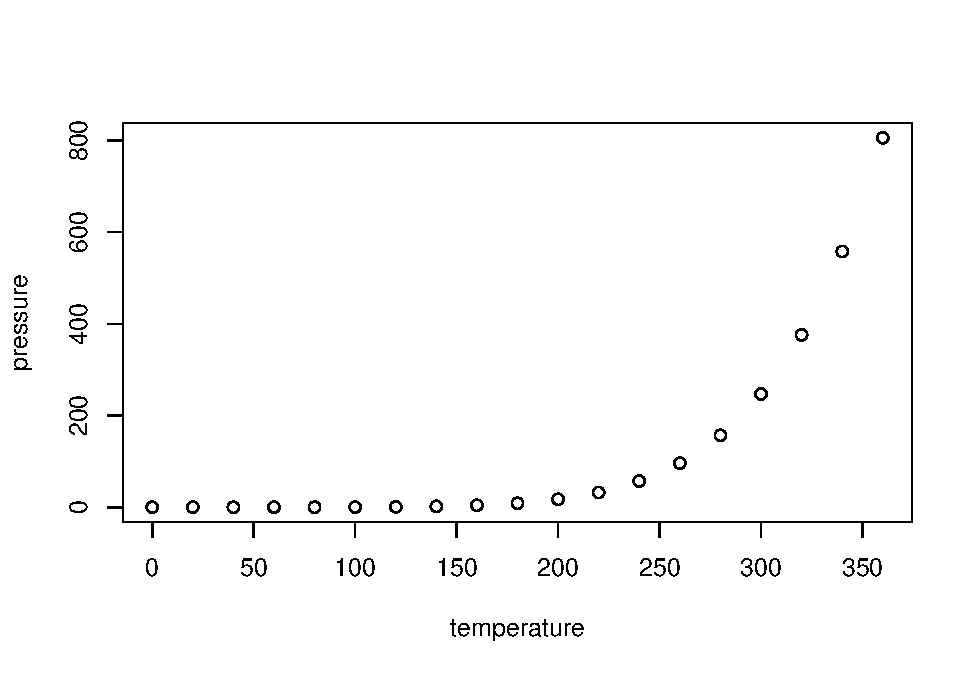
\includegraphics{BP_Rapor_files/figure-latex/pressure-1.pdf}

Note that the \texttt{echo=FALSE} parameter was added to the code chunk to prevent printing of the \textbf{R} code that generated the plot. There are plenty of other ways to add chunk options. More information is available at \url{http://yihui.name/knitr/options/}.

Another useful chunk option is the setting of \texttt{cache=TRUE} as you see here. If document rendering becomes time consuming due to long computations or plots that are expensive to generate you can use knitr caching to improve performance. Later in this file, you'll see a way to reference plots created in \textbf{R} or external figures.

\hypertarget{math-sci}{%
\chapter{Mathematics and Science}\label{math-sci}}

\hypertarget{math}{%
\section{Math}\label{math}}

\TeX~is the best way to typeset mathematics. Donald Knuth designed \TeX~when he got frustrated at how long it was taking the typesetters to finish his book, which contained a lot of mathematics. One nice feature of \emph{R Markdown} is its ability to read LaTeX code directly.

If you are doing a thesis that will involve lots of math, you will want to read the following section which has been commented out. If you're not going to use math, skip over or delete this next commented section.

\hypertarget{birden-fazla-deux11fiux15fim-noktasi-tespiti-multi-change-point-detection}{%
\section{BİRDEN FAZLA DEĞİŞİM NOKTASI TESPİTİ (MULTI CHANGE POINT DETECTION)}\label{birden-fazla-deux11fiux15fim-noktasi-tespiti-multi-change-point-detection}}

Birden fazla değişim noktasının belirlenmesi, bir veri setinde meydana gelen yapısal değişiklikleri tespit etme sürecini ifade eder. Bu analiz, veri setinin farklı segmentlere bölünmesi ve her bir segmentteki değişim noktalarının tanımlanması yoluyla gerçekleştirilir. Değişim noktaları, verinin genel özelliklerinde veya desenlerinde beklenmeyen değişiklikleri temsil eder.

Özellikle zaman serilerinde birden fazla değişim noktasının belirlenmesi, farklı dönemlerde farklı trendlerin veya desenlerin varlığını anlamak açısından önemlidir. Bu tür analizler, endüstriyel süreçlerde, finansal piyasalarda veya epidemiyolojik veriler gibi farklı alanlarda meydana gelen önemli olayları veya dönemleri belirlemek için kullanılabilir.

Bu tür analizler genellikle istatistiksel yöntemler, matematiksel modeller veya makine öğrenimi algoritmaları kullanılarak gerçekleştirilir. Birden fazla değişim noktası tespiti, veri setindeki karmaşık yapısal değişiklikleri belirleme ve anlama amacı taşır. Bu da kullanıcılara önemli olayları tespit etme ve veri setinin farklı bölümlerindeki değişiklikleri anlama imkânı sağlar. Bu analizler, veri setinin farklı segmentlerine ayrılmasını sağlayarak, her bir segmentteki farklı özellikleri ve eğilimleri anlamak için bir yol sunar. Bu da karar verme süreçlerinde daha bilinçli ve stratejik adımlar atılmasına yardımcı olabilir.

Belirli bir zaman serisi veya sinyal akışındaki birden fazla değişim noktasını verimli ve doğru bir şekilde belirleyebilmek için literatürde yaygın olarak kullanılan bir yöntem, maliyet fonksiyonunu (C) minimize ederek birden çok değişim noktasının konumunu belirlemektir. Bu yöntemde, aşırı uyumu önlemek için bir ceza terimi \(\beta f(m)\) ile birlikte maliyet fonksiyonunun toplamı minimize edilmeye çalışılır. Formülü şu şekilde ifade edebiliriz:
\(\sum_{i=1}^{m+1} C(y(\tau_{i-1}+1):\tau_i) + \beta f(m)\)

Bu denklem, değişiklik noktaları (\(y(\tau_{i-1}+1)\) ile
\(\tau_i\) arasındaki segmentler) için maliyet fonksiyonunun toplamını ve aşırı uyumu önlemek için ceza terimini içerir. Bu yöntem, veri setini birden çok bölüme bölmek (maliyet fonksiyonu tarafından belirlenen) ile aşırı karmaşıklığı veya fazla uyumu önlemeye yönelik ceza terimi arasında bir denge kurarak birden fazla değişim noktasını etkili bir şekilde bulmayı amaçlar.

Literatürde birden fazla değişim noktasını belirleme konusunda en yaygın yöntem, bir segment için bir maliyet fonksiyonunu (genellikle negatif log olasılık gibi) minimize etmek ve aşırı uyumlanmayı engellemek için bir ceza terimi (c'nin birden fazla değişim noktası versiyonu olan \(\beta f(m)\)) kullanmaktır. Bu, aynı zamanda benimsediğimiz ve eşlik eden pakette kullandığımız yaklaşımdır. Bu minimize işlemini gerçekleştirmek için bir kaba kuvvet yöntemi, \(2n-1\) çözümü düşünerek, \(m\) bilindiğinde \(n-1\)m'ye indirgenir.

\hypertarget{ikili-segmentasyon-algoritmasux131}{%
\subsection{İkili Segmentasyon Algoritması}\label{ikili-segmentasyon-algoritmasux131}}

İkili segmentasyon algoritması (BinSeg), değişim noktası literatüründe kullanılan en köklü arama yöntemidir. İkili segmentasyon arama algoritmasının erken uygulamaları arasında Scott ve Knott (1974) ile Sen ve Srivastava (1975) bulunmaktadır.

İkili segmentasyon, herhangi bir tek değişim noktası yöntemini ardışık olarak farklı veri setlerinde tekrarlayarak çoklu değişim noktalarına genişletmek için kullanılabilir. İlk olarak, tek bir değişim noktası test istatistiğini tüm veri setine uygular. \(y_{1},y_{2},...,y_{n}\) şeklindeki veri seti üzerinde bir başlangıç noktası belirlenir. Bu başlangıç noktası, veri setinin ortalaması, medyanı veya başka bir özelliği olabilir. Belirlenen başlangıç noktasında bir değişim noktası testi yapılır. Bu test, veri setini iki alt küme olarak böldüğünde, oluşan alt kümelerin toplam maliyetinin belirli bir kritere göre düşük olup olmadığını kontrol eder, yani bir \(\tau\)'nin aşağıdaki koşulu sağlayıp sağlamadığını test eder:

\[C(y_{1:\tau}) + C(y_{(\tau+1):n}) + \beta < C(y_{1:n})\]

Burada:

\begin{itemize}
\item\textbf{C}:Bir segment için maliyet fonksiyonu
\item\textbf{$y_{1:\tau}$}:Başlangıçtan değişim noktasına kadar olan veri seti
\item\textbf{$y_{(\tau+1):n}$}:Değişim noktasından sona kadar olan veri seti
\item\textbf{$\beta$}:Aşırı uyum karşısında koruma sağlayan ceza terimi
\end{itemize}

Eğer bu koşul sağlanmıyorsa, o zaman herhangi bir değişim noktası tespit edilememiştir ve algoritma durur. Aksi takdirde veri, belirlenen değişim noktasından önce ve sonra olmak üzere iki segmente bölünür. Tek değişim noktası tespit yöntemi, değişiklikten önce ve sonra iki yeni segmente de tekrarlanır. Her iki segmentte de değişim noktaları belirlenirse, bunları yeni belirlenen değişim noktasında daha fazla segmentlere böler ve her yeni segmente değişim noktası tespit yöntemini uygular. Bu süreç, verinin herhangi bir bölümünde değişim noktası bulunamayana kadar devam eder.

Çoklu değişim noktalarını belirlemek için yaygın olarak kullanılan bir yaklaşım, aşağıdaki ifadeyi minimize etmektir:

\[\sum_{i=1}^{m+1} C(y(\tau_{i-1}+1):\tau_i) + \beta f(m)\]

Burada, \(C\) bir segment için bir maliyet fonksiyonu ve \(\beta f(m)\) aşırı uyum karşısında koruma sağlayan bir ceza terimidir.

İkili segmentasyon, herhangi bir değişim noktasının konumu önceden belirlenmiş değişim noktalarına bağlı olduğu için (\(f(m) = m\) olarak) yukarıdaki denklemin yaklaşık bir minimize edilmesidir. Algoritmanın her adımı, bu denklemi azaltıyorsa ek bir değişim noktası eklemeye çalışır. İkili segmentasyon algoritmasının avantajı, \(n\)'nin veri uzunluğu olduğu durumda \(O(n)\) hesaplama maliyeti ile uygulanabilen hızlı bir algoritma olmasıdır. Ancak, \(C\)'yi uygun bir şekilde seçmek zor olabilir ve farklı \(C\) seçimleri, değişim noktalarının sayısının tahmininde önemli farklara neden olabilir.

\hypertarget{pelt}{%
\subsection{PELT}\label{pelt}}

\hypertarget{paruxe7alux131-regresyon}{%
\subsection{Parçalı Regresyon}\label{paruxe7alux131-regresyon}}

Parçalı veya kesik çizgili modeller, yanıt ile bir veya daha fazla açıklayıcı değişken arasındaki ilişkilerin parçalı doğrusal olduğu, yani iki veya daha fazla değişkenle temsil edildiği regresyon modelleridir.Bu ilişkiler, genellikle bilinmeyen değerlerde birleştirilen iki veya daha fazla düz çizgi tarafından temsil edilir, bu değerlere genellikle kırılma noktaları, değişim noktaları veya birleşim noktaları denir. Bu yöntemde bağımsız değişken, aralıklara bölünür ve her bir aralığa ayrı bir çizgi segmenti uyarlanır.Parçalı regresyon analizi ayrıca çeşitli bağımsız değişkenlerle yapılan çok değişkenli veriler üzerinde de gerçekleştirilebilir. Parçalı regresyon analizi, bağımsız değişkenlerin belirli gruplara ayrıldığı durumlarda, bu gruplardaki değişkenler arasındaki ilişkilerin farklı olduğuna inanıldığında kullanışlıdır. Bu parçalar arasındaki sınırlar, değişim noktaları olarak adlandırılır.

Matematiksel olarak, model şu şekilde ifade edilebilir:

\(y = \beta_{0i} + \beta_{1i} x + \epsilon\)

Bu denklemde, \(\beta_{0i}\) ve \(\beta_{1i}\) sırasıyla i-inci segmentin kesişim noktası ve eğimini temsil eder.

Parçalı regresyon, ekonomi, biyoloji, çevre bilimleri, epidemiyoloji gibi çeşitli alanlarda kullanılır.Kalite iyileştirme müdahaleleriyle ilgili çalışmalarda parçalı regresyon analizlerinin kullanımına dair birçok örnek yayınlanmıştır.

Temel bir parçalı regresyon analizinde zaman periyodu müdahale öncesi ve sonrası parçalara bölünür ve her parçada ayrı ayrı kesişme noktaları ve eğimler tahmin edilir. Müdahaleden önce ve sonra kesişmelerde ve eğimlerdeki değişiklikleri test etmek için istatistiksel testler gerçekleştirilir. Veriler ve model spesifikasyonunda bazı basit değişikliklerle parçalı regresyon analizi, genellikle standart istatistiksel yazılım paketlerinde kolayca uygulanabilir. Genellikle, zaman içinde alınan gözlemler ilişkilidir, bu nedenle otokorelasyonu hesaba katmak için genellikle ek bir düzeltme yapılması gerekir.

Parçalı doğrusal regresyon, parçalı regresyonun doğrusal regresyon kullanılarak elde edilen bir alt türüdür.İki parçalı doğrusal regresyon, bir değişim noktası ile ayrılmış iki parçayla, değişken bir etkenin (x) yanıt fonksiyonunun (\(Y_{r}\)) ani bir değişikliğini nicelendirmek için kullanışlı olabilir. Değişim noktası, yanıt fonksiyonunun kritik, güvenli veya eşik değeri olarak yorumlanabilir; bu değerin ötesinde veya altında (istenmeyen) etkiler meydana gelebilir. Değişim noktası, karar verme süreçlerinde önemlidir.

Her bir parça için ayrı ayrı uygulanan en küçük kareler yöntemi, iki regresyon çizgisini veriye mümkün olduğunca iyi uyacak şekilde oluştururken, gözlemlenen (y) ve hesaplanan (Yr) bağımlı değişken değerleri arasındaki farkın karesini en aza indirir. Bu yöntemle şu iki denklem elde edilir:

\(Yr = A1.x+K1 <BP\) (değişim noktası için)

\(Yr = A2.x+K2 >BP\) (değişim noktası için)

Burada:

\begin{itemize}
\item $Y_{r}$, x'in belirli bir değeri için beklenen (tahmin edilen) y değeridir;
\item A1 ve A2 regresyon katsayılarıdır (çizgi segmentinin eğimini gösterir);
\item K1 ve K2 regresyon sabitleridir (y-ekseninde kesişimi gösterir).
\end{itemize}

Bu yöntem aynı zamanda iki korelasyon katsayısı (R) da üretir:

\(R_{1}^{2}=1-{\frac {\sum (y-Y_{r})^{2}}{\sum (y-Y_{a1})^{2}}}\) x\textless BP (değişim noktası için)

ve

\(R_{2}^{2}=1-{\frac {\sum (y-Y_{r})^{2}}{\sum (y-Y_{a2})^{2}}}\) x\textgreater BP (değişim noktası için)

Burada:

\begin{itemize}
\item $\sum (y-Y_{r})^{2}$  her bir parça için minimize edilmiş SSD'yi temsil eder
\item $Y_{a1}$ ve $Y_{a2}$ ilgili parçalarda y'nin ortalamasıdır.
\end{itemize}

En uygun eğilimi belirlemede, bu eğilimin güvenilir (anlamlı) olduğundan emin olmak için istatistiksel testler gerçekleştirilmelidir.

Eğer anlamlı bir değişim noktası tespit edilemezse, değişim noktası olmadan bir regresyona geçilmelidir.
Aşağıdaki istatistiksel testler, eğilim türünü belirlemek için kullanılır:

\begin{enumerate}
\item\textbf{A1 ve A2'nin Anlamlılığı:} A1 ve A2'nin anlamlılığı, A1 ve A2'nin standart hata SE'si ve Student'ün t-distribution'ı kullanılarak belirlenir.
\item\textbf{A1 ve A2'nin Farkının Anlamlılığı:} A1 ve A2'nin farkının anlamlılığı, farklarının standart hatası SE ve Student'ün t-distribution'ı kullanılarak belirlenir.
\item\textbf{Y1 ve Y2'nin Farkının Anlamlılığı:} Y1 ve Y2'nin farkının anlamlılığı, farklarının standart hatası SE ve Student'ün t-distribution'ı kullanılarak belirlenir.
\item\textbf{Değişim Noktasının Varlığını Test Etme:} Sözde skor testi, parçalı çizginin tahminini gerektirmez ve kırılma noktasının varlığını test etmek için daha formal bir istatistiksel yaklaşımdır.
\end{enumerate}

Ayrıca, tüm verilerin korelasyon katsayısı (\(R_{a}\)), belirleme katsayısı veya açıklama katsayısı, regresyon fonksiyonlarının güven aralıkları ve ANOVA analizi kullanılmaktadır.

\(C_{d}\) katsayısı, tüm veri seti için belirlenen şartlar altında maksimize edilmesi gereken bir belirleme katsayısıdır ve şu formülle hesaplanır:

\(C_{d}=1-{\sum (y-Y_{r})^{2} \over \sum (y-Y_{a})^{2}}\)

Burada \(Y_{r}\), önceki regresyon denklemlerine göre beklenen (tahmin edilen) y değeridir ve \(Y_{a}\), tüm y değerlerinin ortalamasıdır.

\(C_{d}\) katsayısı, 0 ile 1 arasında değer alır. Saf, parçalanmamış doğrusal regresyonda, \(C_{d}\) ve \(R_{a}^2\) değerleri eşittir. Parçalı regresyonda, \(C_{d}\)'nin \(R_{a}^2\)'den anlamlı derecede büyük olması, parçalanmanın haklı olduğunu gösterir.

Değişim noktasının en uygun değeri, \(C_{d}\) katsayısının maksimum olduğu noktada bulunabilir.

You may wish to put your reaction in an equation environment, which means that LaTeX will place the reaction where it fits and will number the equations for you.

\begin{equation}
  \mathrm{C_6H_{12}O_6  + 6O_2} \longrightarrow \mathrm{6CO_2 + 6H_2O}
  \label{eq:reaction}
\end{equation}

We can reference this combustion of glucose reaction via Equation \eqref{eq:reaction}.

\hypertarget{other-examples-of-reactions}{%
\subsection{Other examples of reactions}\label{other-examples-of-reactions}}

\(\mathrm{NH_4Cl_{(s)}}\) \(\rightleftharpoons\) \(\mathrm{NH_{3(g)}+HCl_{(g)}}\)

\noindent \(\mathrm{MeCH_2Br + Mg}\) \(\xrightarrow[below]{above}\) \(\mathrm{MeCH_2\bullet Mg \bullet Br}\)

\hypertarget{Bolum3}{%
\chapter{Bölüm 3 Başlık}\label{Bolum3}}

\hypertarget{bu-bir-alt-baux15flux131k}{%
\section{Bu bir alt başlık}\label{bu-bir-alt-baux15flux131k}}

Bu bölümde şu konular yer almaktadır\ldots{}

\hypertarget{bu-ikinci-seviye-bir-alt-baux15flux131k}{%
\subsection{Bu ikinci seviye bir alt başlık}\label{bu-ikinci-seviye-bir-alt-baux15flux131k}}

\hypertarget{Bolum4}{%
\chapter{Bölüm 4 Başlık}\label{Bolum4}}

\hypertarget{bu-bir-alt-baux15flux131k-1}{%
\section{Bu bir alt başlık}\label{bu-bir-alt-baux15flux131k-1}}

Bu bölümde şu konular yer almaktadır\ldots{}

\hypertarget{bu-ikinci-seviye-bir-alt-baux15flux131k-1}{%
\subsection{Bu ikinci seviye bir alt başlık}\label{bu-ikinci-seviye-bir-alt-baux15flux131k-1}}

\hypertarget{sonuuxe7}{%
\chapter*{Sonuç}\label{sonuuxe7}}
\addcontentsline{toc}{chapter}{Sonuç}

If we don't want Conclusion to have a chapter number next to it, we can add the \texttt{\{-\}} attribute.

\textbf{More info}

And here's some other random info: the first paragraph after a chapter title or section head \emph{shouldn't be} indented, because indents are to tell the reader that you're starting a new paragraph. Since that's obvious after a chapter or section title, proper typesetting doesn't add an indent there.

\hypertarget{kaynaklar}{%
\chapter*{Kaynaklar}\label{kaynaklar}}
\addcontentsline{toc}{chapter}{Kaynaklar}

\markboth{Kaynaklar}{Kaynaklar}

\hypertarget{refs}{}
\begin{CSLReferences}{1}{0}
\leavevmode\vadjust pre{\hypertarget{ref-angel2000}{}}%
Angel, E. (2000). \emph{Interactive Computer Graphics : A Top-Down Approach with OpenGL}. Boston, MA: Addison Wesley Longman.

\leavevmode\vadjust pre{\hypertarget{ref-angel2001a}{}}%
Angel, E. (2001a). \emph{Batch-file Computer Graphics : A Bottom-Up Approach with QuickTime}. Boston, MA: Wesley Addison Longman.

\leavevmode\vadjust pre{\hypertarget{ref-angel2001b}{}}%
Angel, E. (2001b). \emph{test second book by angel}. Boston, MA: Wesley Addison Longman.

\leavevmode\vadjust pre{\hypertarget{ref-birge2007}{}}%
Birgé, L. ve Massart, P. (2007). Minimal penalties for Gaussian model selection. \emph{Probability theory and related fields}, \emph{138}, 33-73.

\leavevmode\vadjust pre{\hypertarget{ref-chen2000}{}}%
Chen, J., Gupta, A. K. ve Gupta, A. (2000). \emph{Parametric statistical change point analysis} (C. 192). Springer.

\leavevmode\vadjust pre{\hypertarget{ref-deussen2000}{}}%
Deussen, O. ve Strothotte, T. (2000). Computer-Generated Pen-and-Ink Illustration of Trees. \emph{{``Proceedings of''} SIGGRAPH 2000}, Computer Graphics Proceedings, Annual Conference Series, 13-18.

\leavevmode\vadjust pre{\hypertarget{ref-hipr1997}{}}%
Fisher, R., Perkins, S., Walker, A. ve Wolfart, E. (1997). \emph{Hypermedia Image Processing Reference}. New York, NY: John Wiley \& Sons.

\leavevmode\vadjust pre{\hypertarget{ref-goochandgooch2001}{}}%
Gooch, B. ve Gooch, A. (2001a). \emph{{Non-Photorealistic Rendering}}. Natick, Massachusetts: A K Peters.

\leavevmode\vadjust pre{\hypertarget{ref-goochandgooch2001a}{}}%
Gooch, B. ve Gooch, A. (2001b). \emph{Test second book by gooches}. Natick, Massachusetts: A K Peters.

\leavevmode\vadjust pre{\hypertarget{ref-guyon1999}{}}%
Guyon, X. ve Yao, J. (1999). On the underfitting and overfitting sets of models chosen by order selection criteria. \emph{Journal of Multivariate Analysis}, \emph{70}(2), 221-249.

\leavevmode\vadjust pre{\hypertarget{ref-hertzmann2000}{}}%
Hertzmann, A. ve Zorin, D. (2000). Illustrating Smooth Surfaces. \emph{Proceedings of SIGGRAPH 2000}, Computer Graphics Proceedings, Annual Conference Series, \emph{5}(17), 517-526.

\leavevmode\vadjust pre{\hypertarget{ref-hinkley1970}{}}%
Hinkley, D. V. (1970). Inference about the change-point in a sequence of random variables.

\leavevmode\vadjust pre{\hypertarget{ref-jain1989}{}}%
Jain, A. K. (1989). \emph{Fundamentals of Digital Image Processing}. Englewood Cliffs, New Jersey: Prentice-Hall.

\leavevmode\vadjust pre{\hypertarget{ref-jengupta1987}{}}%
Jen, T. ve Gupta, A. K. (1987). On testing homogeneity of variances for Gaussian models. \emph{Journal of Statistical Computation and Simulation}, \emph{27}(2), 155-173.

\leavevmode\vadjust pre{\hypertarget{ref-lavielle2005}{}}%
Lavielle, M. (2005). Using penalized contrasts for the change-point problem. \emph{Signal processing}, \emph{85}(8), 1501-1510.

\leavevmode\vadjust pre{\hypertarget{ref-Molina1994}{}}%
Molina, S. T. ve Borkovec, T. D. (1994). The {P}enn {S}tate Worry Questionnaire: Psychometric properties and associated characteristics. G. C. L. Davey ve F. Tallis (Ed.), \emph{Worrying: Perspectives on theory, assessment and treatment} içinde (ss. 265-283). New York: Wiley.

\leavevmode\vadjust pre{\hypertarget{ref-noble2002}{}}%
Noble, S. G. (2002). \emph{Turning images into simple line-art}. (Yayımlanmamış undergraduate thesis). Reed College.

\leavevmode\vadjust pre{\hypertarget{ref-reedweb2007}{}}%
Reed~College. (2007). LaTeX Your Document. \url{http://web.reed.edu/cis/help/LaTeX/index.html} adresinden erişildi.

\leavevmode\vadjust pre{\hypertarget{ref-russ1995}{}}%
Russ, J. C. (1995). \emph{{The Image Processing Handbook, Second Edition}}. Boca Raton, Florida: CRC Press.

\leavevmode\vadjust pre{\hypertarget{ref-salisbury1997}{}}%
Salisbury, M. P., Wong, M. T., Hughes, J. F. ve Salesin, D. H. (1997). Orientable Textures for Image-Based Pen-and-Ink Illustration. \emph{{``Proceedings of''} SIGGRAPH 97}, Computer Graphics Proceedings, Annual Conference Series, 401-406.

\leavevmode\vadjust pre{\hypertarget{ref-savitch2001}{}}%
Savitch, W. (2001). \emph{JAVA: An Introduction to Computer Science \& Programming}. Upper Saddle River, New Jersey: Prentice Hall.

\leavevmode\vadjust pre{\hypertarget{ref-tukey1984}{}}%
Tukey, J. W. (1984). \emph{The collected works of John W. Tukey} (C. 1). Taylor \& Francis.

\leavevmode\vadjust pre{\hypertarget{ref-wong1999}{}}%
Wong, E. (1999). \emph{{Artistic Rendering of Portrait Photographs}}. (Yayımlanmamış mathesis). Cornell University.

\end{CSLReferences}

\setlength{\parindent}{-0.20in}
\setlength{\leftskip}{0.20in}
\setlength{\parskip}{8pt}

\appendix

\hypertarget{ilk-ek-baux15flux131ux11fux131}{%
\chapter{İlk Ek Başlığı}\label{ilk-ek-baux15flux131ux11fux131}}

This first appendix includes all of the R chunks of code that were hidden throughout the document (using the \texttt{include\ =\ FALSE} chunk tag) to help with readibility and/or setup.

\textbf{In the main Rmd file}

\begin{Shaded}
\begin{Highlighting}[]
\CommentTok{\# This chunk ensures that the thesisdown package is}
\CommentTok{\# installed and loaded. This thesisdown package includes}
\CommentTok{\# the template files for the thesis.}
 \ControlFlowTok{if}\NormalTok{(}\SpecialCharTok{!}\FunctionTok{require}\NormalTok{(remotes)) }\FunctionTok{install.packages}\NormalTok{(}\StringTok{"remotes"}\NormalTok{, }\AttributeTok{repos =} \StringTok{"http://cran.rstudio.com"}\NormalTok{)}
 \ControlFlowTok{if}\NormalTok{(}\SpecialCharTok{!}\FunctionTok{require}\NormalTok{(thesisdown))remotes}\SpecialCharTok{::}\FunctionTok{install\_github}\NormalTok{(}\StringTok{"ismayc/thesisdown"}\NormalTok{)}
 \FunctionTok{library}\NormalTok{(thesisdown)}
\end{Highlighting}
\end{Shaded}

\textbf{In Chapter \ref{ref-labels}:}

\hypertarget{ikinci-ek-baux15flux131ux11fux131}{%
\chapter{İkinci Ek Başlığı}\label{ikinci-ek-baux15flux131ux11fux131}}

İkinci Ek




\end{document}
